\documentclass[tt2]{penoverslag}

%%% PACKAGES
\renewcommand{\refname}{}
\usepackage{lipsum}
\usepackage{gensymb}
\usepackage [dutch] {babel}
\usepackage{graphicx}
\usepackage{amsmath}
\usepackage{listings}
\usepackage{subcaption}
\usepackage{lscape}
\usepackage[absolute]{textpos}
  \setlength{\TPHorizModule}{1cm}
  \setlength{\TPVertModule}{1cm}


\begin{document}

\team{Zilver} % teamkleur
\members{Sam Gielis\\
         Sophie Marien\\
         Toon Nolten\\
         Nele Rober\\
         Gerlinde Van Roey\\
         Maxim Van Mechelen} % teamleden

\maketitlepage

\tableofcontents
\newpage

\begin{abstract}
Het P\&O-project heeft als doel vier autonome robots \textit{Team Treasure Trek} te laten spelen. Dit verslag beschrijft de invulling die team Zilver aan het project gaf.\\

De robot is voorzien van een lichtsensor, een infraroodsensor en een ultrasone sensor. Verder is de robot voorzien van een schep waarmee hij het voorwerp kan oprapen.\\

De robot kan een doolhof verkennen en hiervan een map bijhouden. Wanneer hij een tegel vindt die mogelijk een voorwerp bevat, zal het nakijken van deze tegel prioriteit krijgen. Via RabbitMQ kunnen de robots en simulators met elkaar communiceren. Zo kunnen de duo's een plaats afspreken om elkaar te ontmoeten.\\

Een computerprogramma simuleert de werking van robots. Deze simulator kan vier robots tegelijk simuleren of kan in hybride vorm gebruikt worden (waarbij bijvoorbeeld \'e\'en fysieke en drie virtuele robots gebruikt worden). De gesimuleerde robots gedragen zich volledig analoog aan de fysieke robot.
\end{abstract}

\setcounter{tocdepth}{2}
\tableofcontents
%figuur robot
\begin{figure}[!hb]
\begin{textblock}{38}(4.5,15.5)
    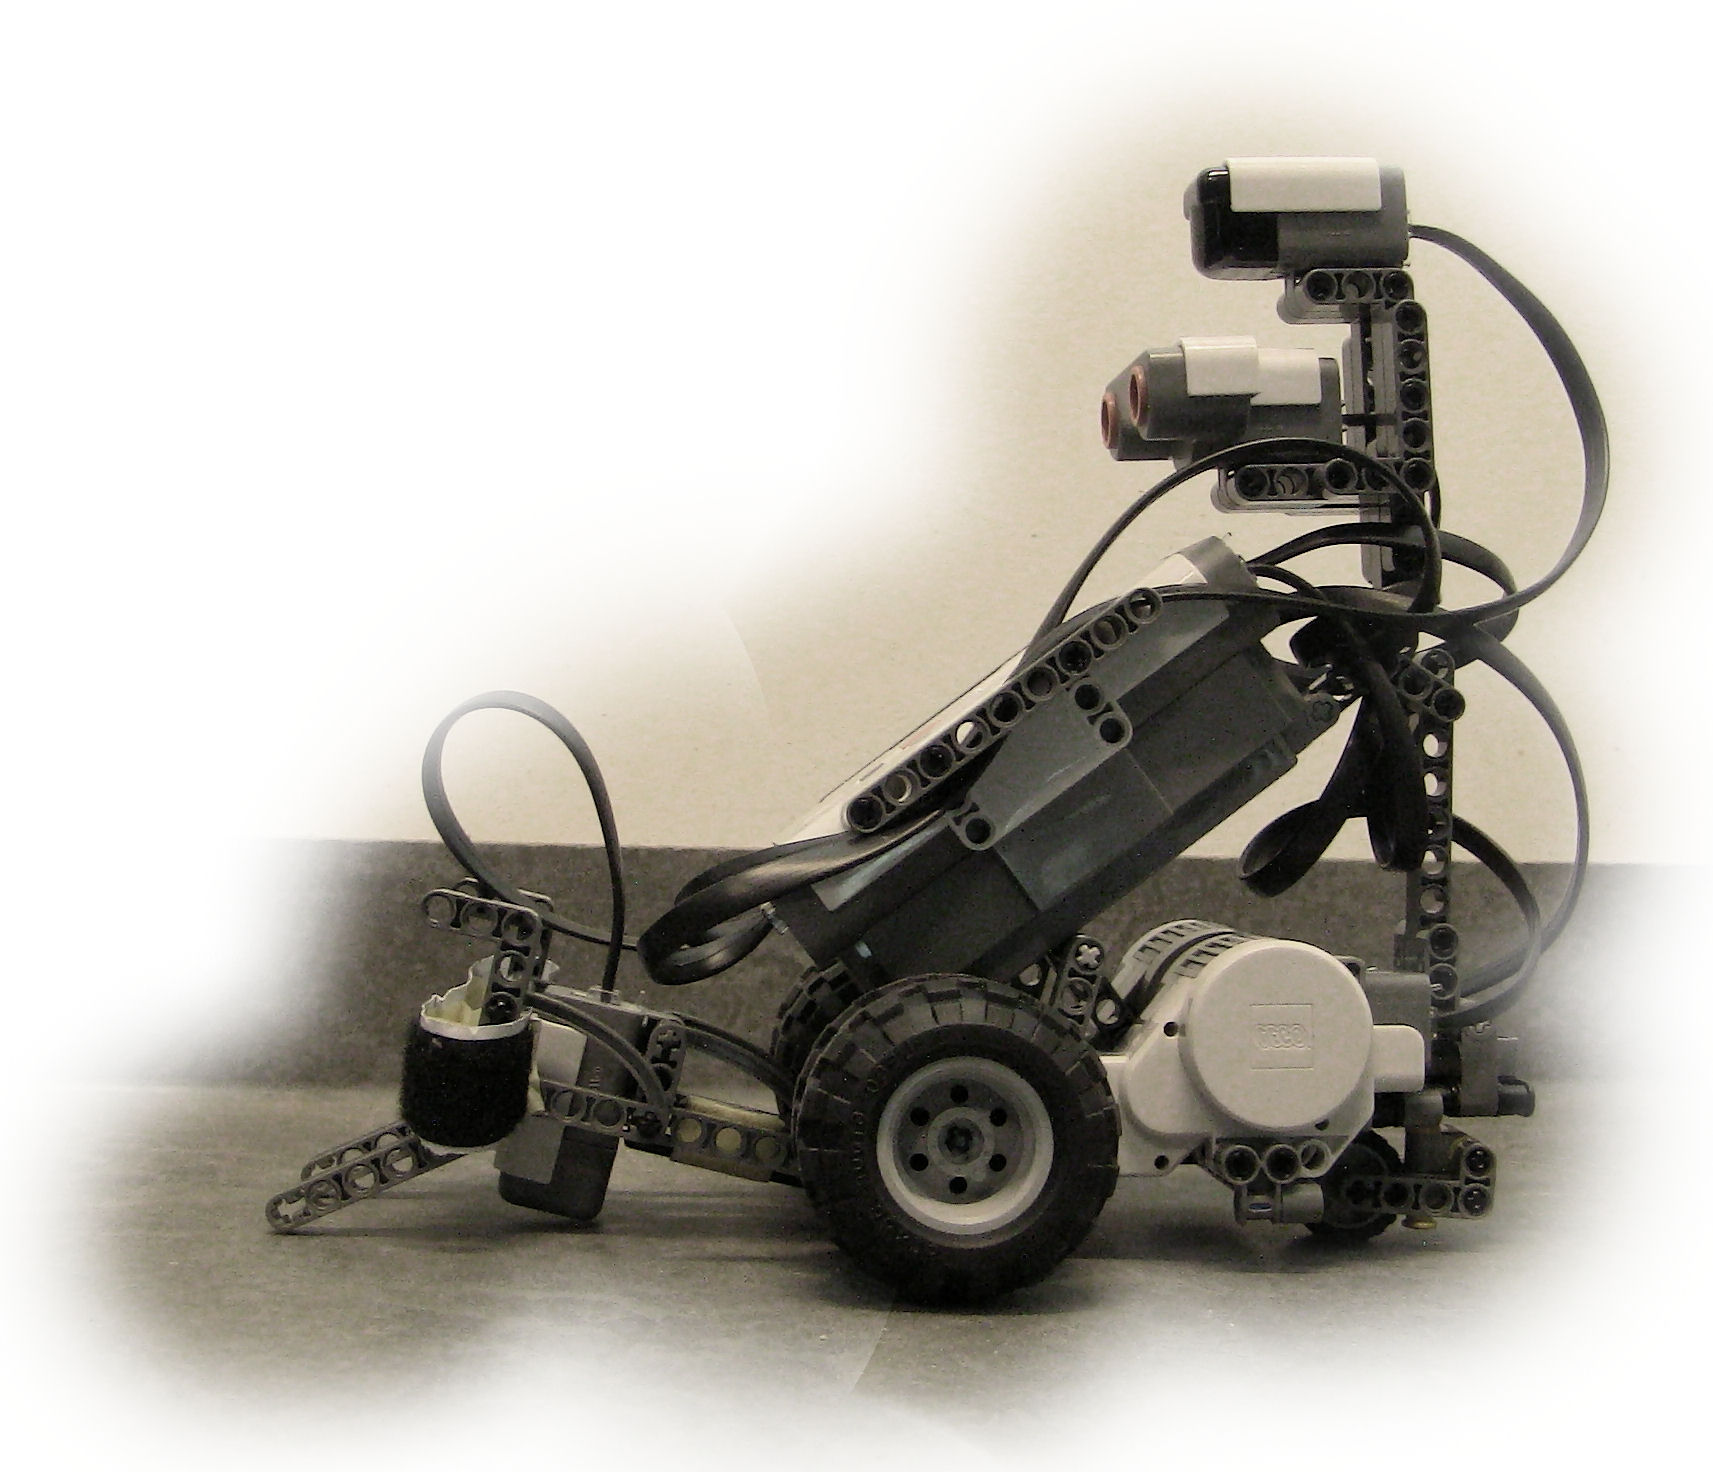
\includegraphics[width=0.5\textwidth]{robotFP}
    \label{fig:robotFP2}
\end{textblock}
\end{figure}

\newpage


% == INLEIDING == %
\section{Inleiding} % 4 ok
\label{ssec:inl}
In het kader van het vak `Probleemoplossen en Ontwerpen: computerwetenschappen' wordt gewerkt rond autonome intelligente robots. Verschillende teams bouwen en programmeren een robot met behulp van LEGO Mindstorms. Deze robot moet uiteindelijk samen met drie andere robots volledig autonoom \textit{Team Treasure Trek} kunnen spelen.
De robots moeten hierbij in een onbekend doolhof op zoek naar een bepaald voorwerp (een wc-rol). Elke robot krijgt zijn eigen voorwerp toegewezen. Wanneer een robot zijn voorwerp gevonden heeft, komt hij te weten met welke robot hij moet samenwerken. Elk duo moet beide voorwerpen bij elkaar brengen. Het duo dat hier eerst in slaagt, wint.\\

Voor de tweede demonstratie wordt met \'e\'en fysieke en drie gesimuleerde robots gewerkt. Het is ook mogelijk met vier virtuele robots te werken. De doolhof bevat mogelijk een wip. De robots zijn in staat hun eigen voorwerp te vinden en op te rapen. Wanneer een robot weet wie zijn teamgenoot is, kan hij hiermee een punt afspreken om samen te komen.\\


\section{Bouw robot}
\label{ssec:bouwrob}
LEGO Mindstorms  biedt een bouwpakket voor een robot aan. Een NXT-microcomputer laat toe de robot te programmeren. Met behulp van leJOS  kan dit in Java.

De robot moet in staat zijn een wc-rolletje, op te nemen. Verder moet de robot andere robots en de stand van de wip kunnen detecteren.

\subsection{Fysieke bouw}
\label{ssec:fysb}
Een infraroodsensor werd gemonteerd bovenop de robot. Wanneer een infraroodbal onder een wip geplaatst wordt, kan de robot bepalen of de wip naar beneden staat. In dat geval wordt het infrarood licht immers geblokt. Later kan de infraroodsensor eventueel gebruikt worden om robots te detecteren.\\

Het voorwerp kan op verschillende manieren worden opgeraapt. Enkele opties werden getest: een schep met motor achteraan, een kartonnen schep vooraan en een plastieken schep met klittenband vooraan. Figuur \ref{fig:robotBouw} geeft deze opstellingen weer. Volgende bevindingen werden gemaakt:

\begin{enumerate}
\item De robot heft het voorwerp expliciet op met behulp van een extra motor. Deze opstelling maakte de robot te lang waardoor hij moeilijk kon draaien zonder tegen een muur te botsen. Er werd besloten de schep vooraan te plaatsen.
\item Vooraan is niet genoeg plaats voor een extra motor, deze werd niet gebruikt. Een halve wc-rol leek een ideale vorm voor de schep. Na testen bleek dit echter niet altijd te werken.
\item De robot neemt het voorwerp op met behulp van klittenband. De schep zorgt ervoor dat het voorwerp niet over de grond sleept. Zo zit het niet in de weg voor de wip. Dit is de huidige opstelling.
\end{enumerate}

De infrarood- en ultrasone sensor worden vast gemonteerd op de robot.
De schep werd samen met de lichtsensor gemonteerd op een hefboomsysteem. Wanneer de robot over de wip rijdt, gaat dit systeem omhoog. Zo botsen er geen onderdelen tegen de wip.

De robot is ook voorzien van een dubbel paar wielen. Dit vermijdt dat hij gaat schuiven op de wip.

Figuur \ref{fig:robotDetail} geeft details van de schep, de wielen en de sensoren.

% bouw robot
\begin{figure}
\centering
	\begin{subfigure}[h]{0.33\textwidth}
	\centering
		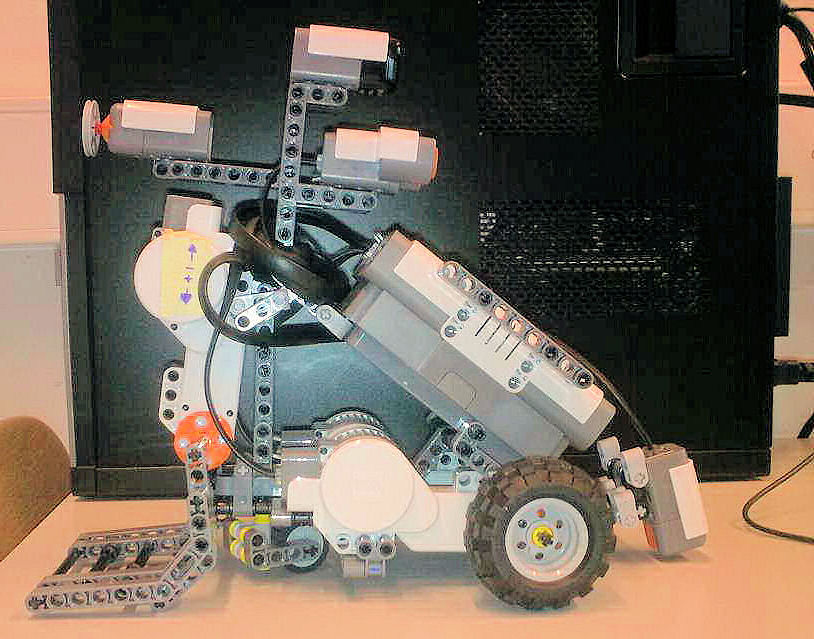
\includegraphics[width=\textwidth]{robotOud1}
		\caption{opstelling 1}
	\end{subfigure}%
	\begin{subfigure}[h]{0.33\textwidth}
		\centering
		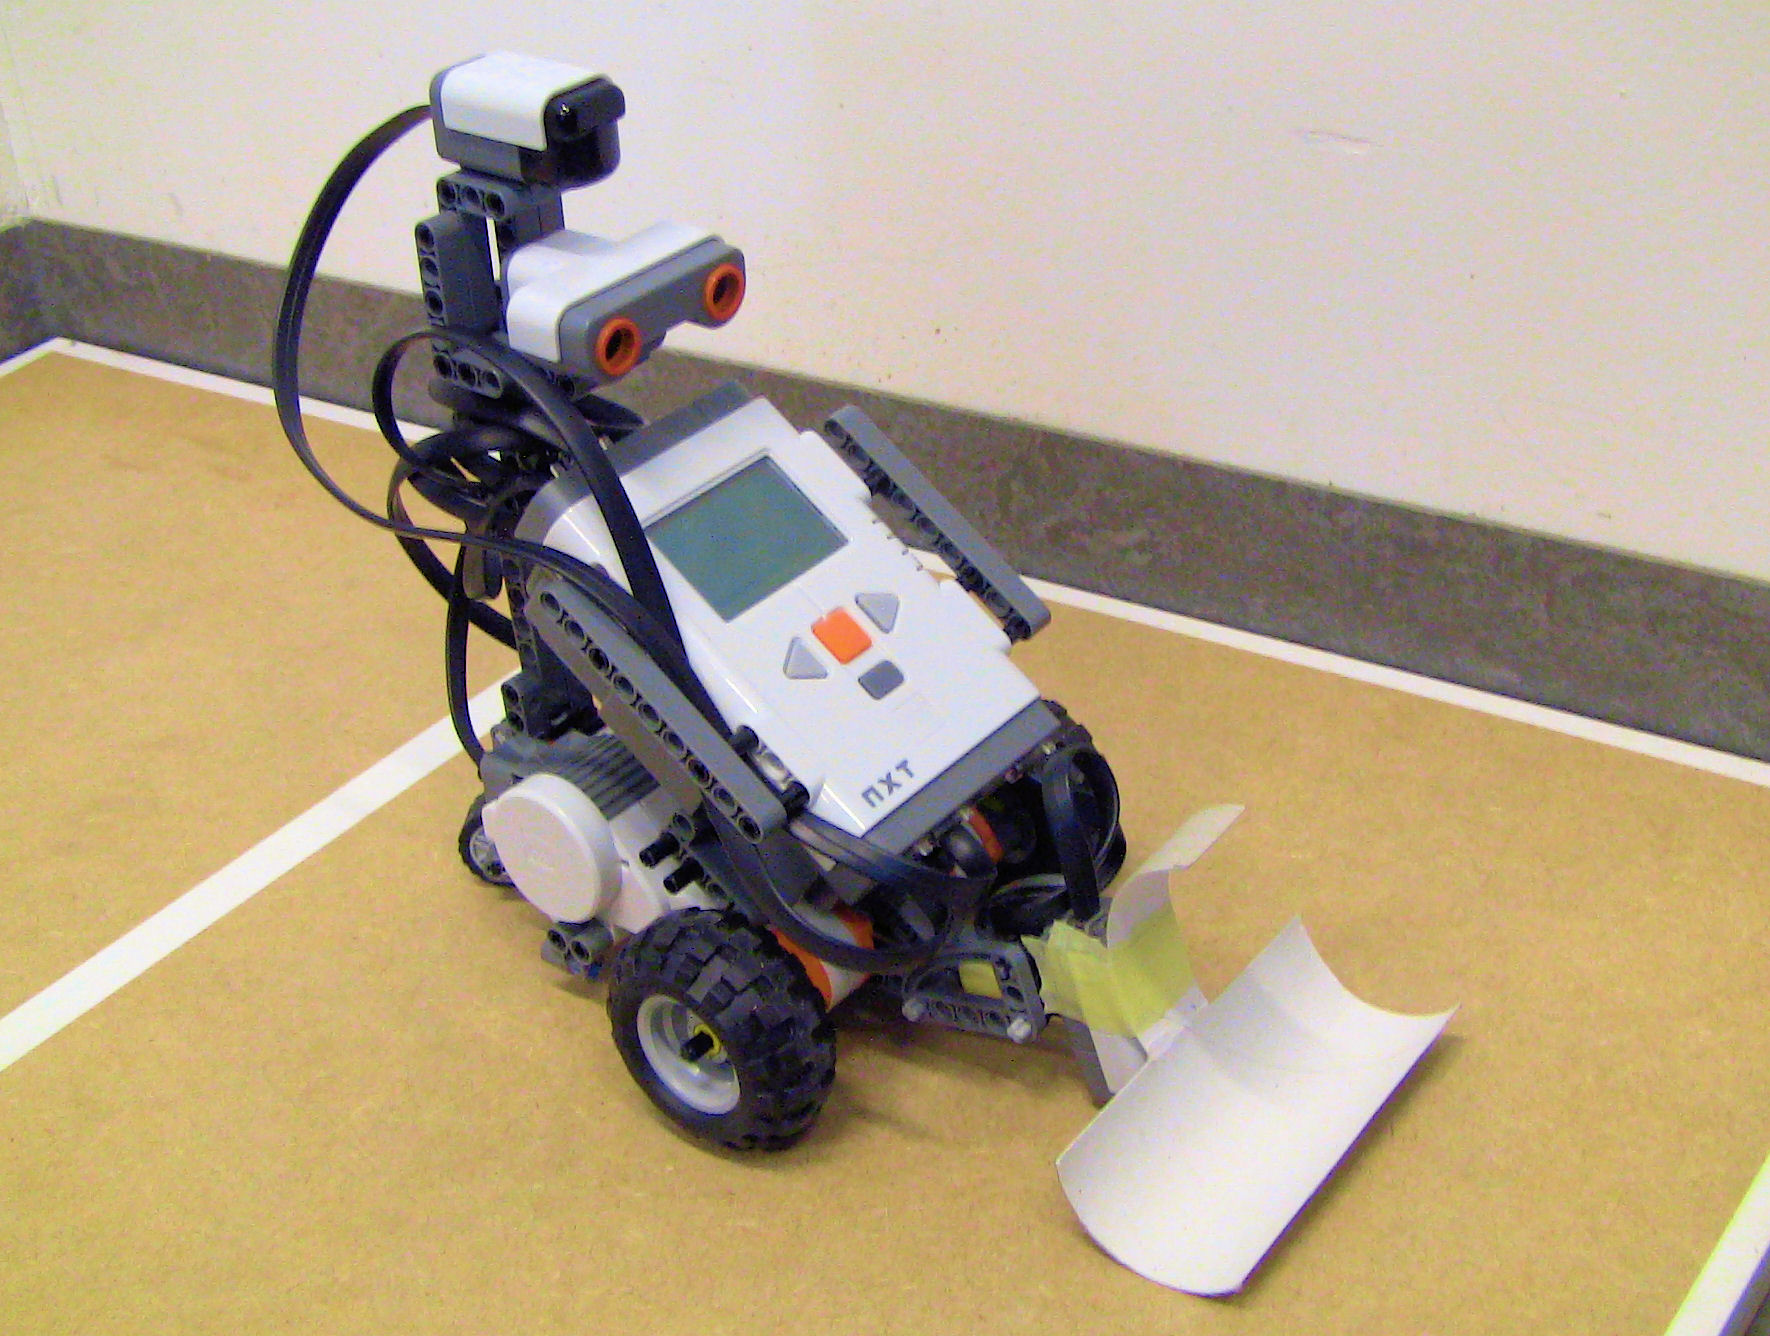
\includegraphics[width=\textwidth]{robotOud2}
	\caption{opstelling 2}
	\end{subfigure}
	\begin{subfigure}[h]{0.33\textwidth}
		\centering
		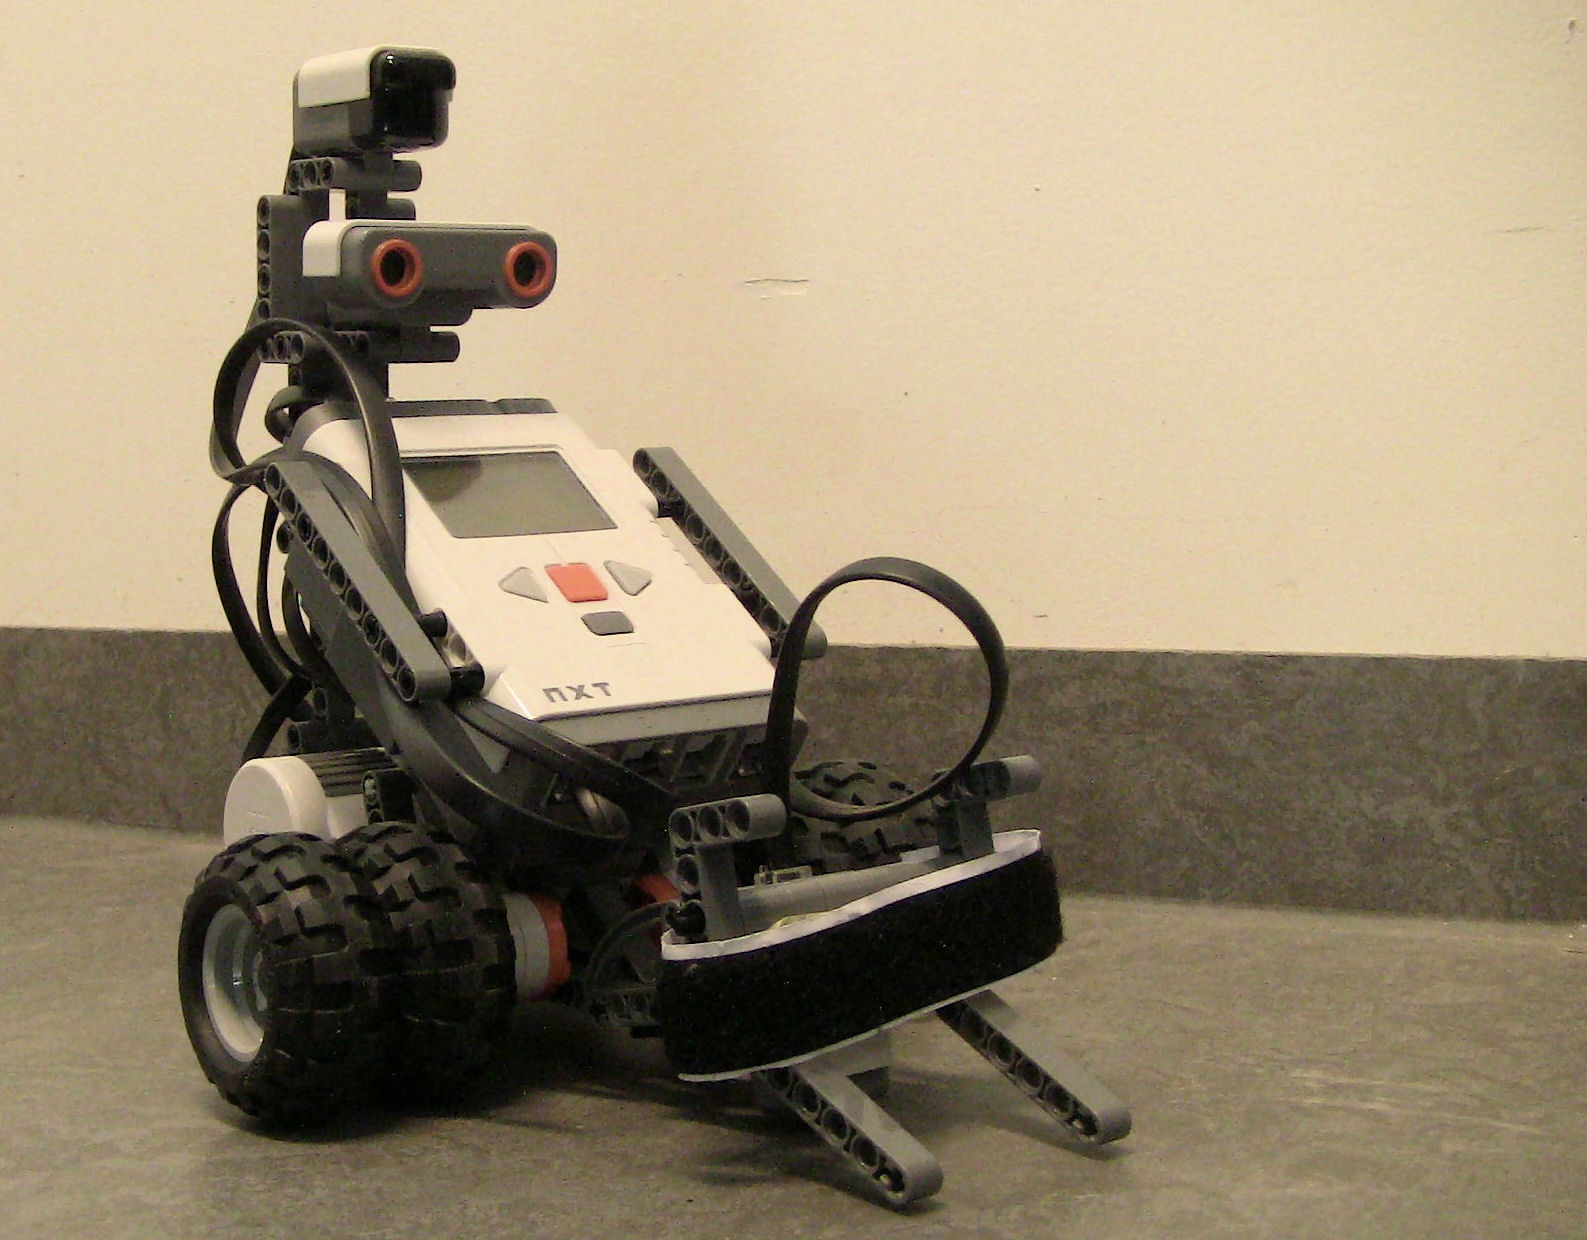
\includegraphics[width=\textwidth]{robotNieuw}
	\caption{opstelling 3}
	\end{subfigure}
\caption{Een vergelijking tussen verschillende ontwerpen.}
\label{fig:robotBouw}
\end{figure}

% details robot
\begin{figure}
\centering
	\begin{subfigure}[h]{0.33\textwidth}
	\centering
		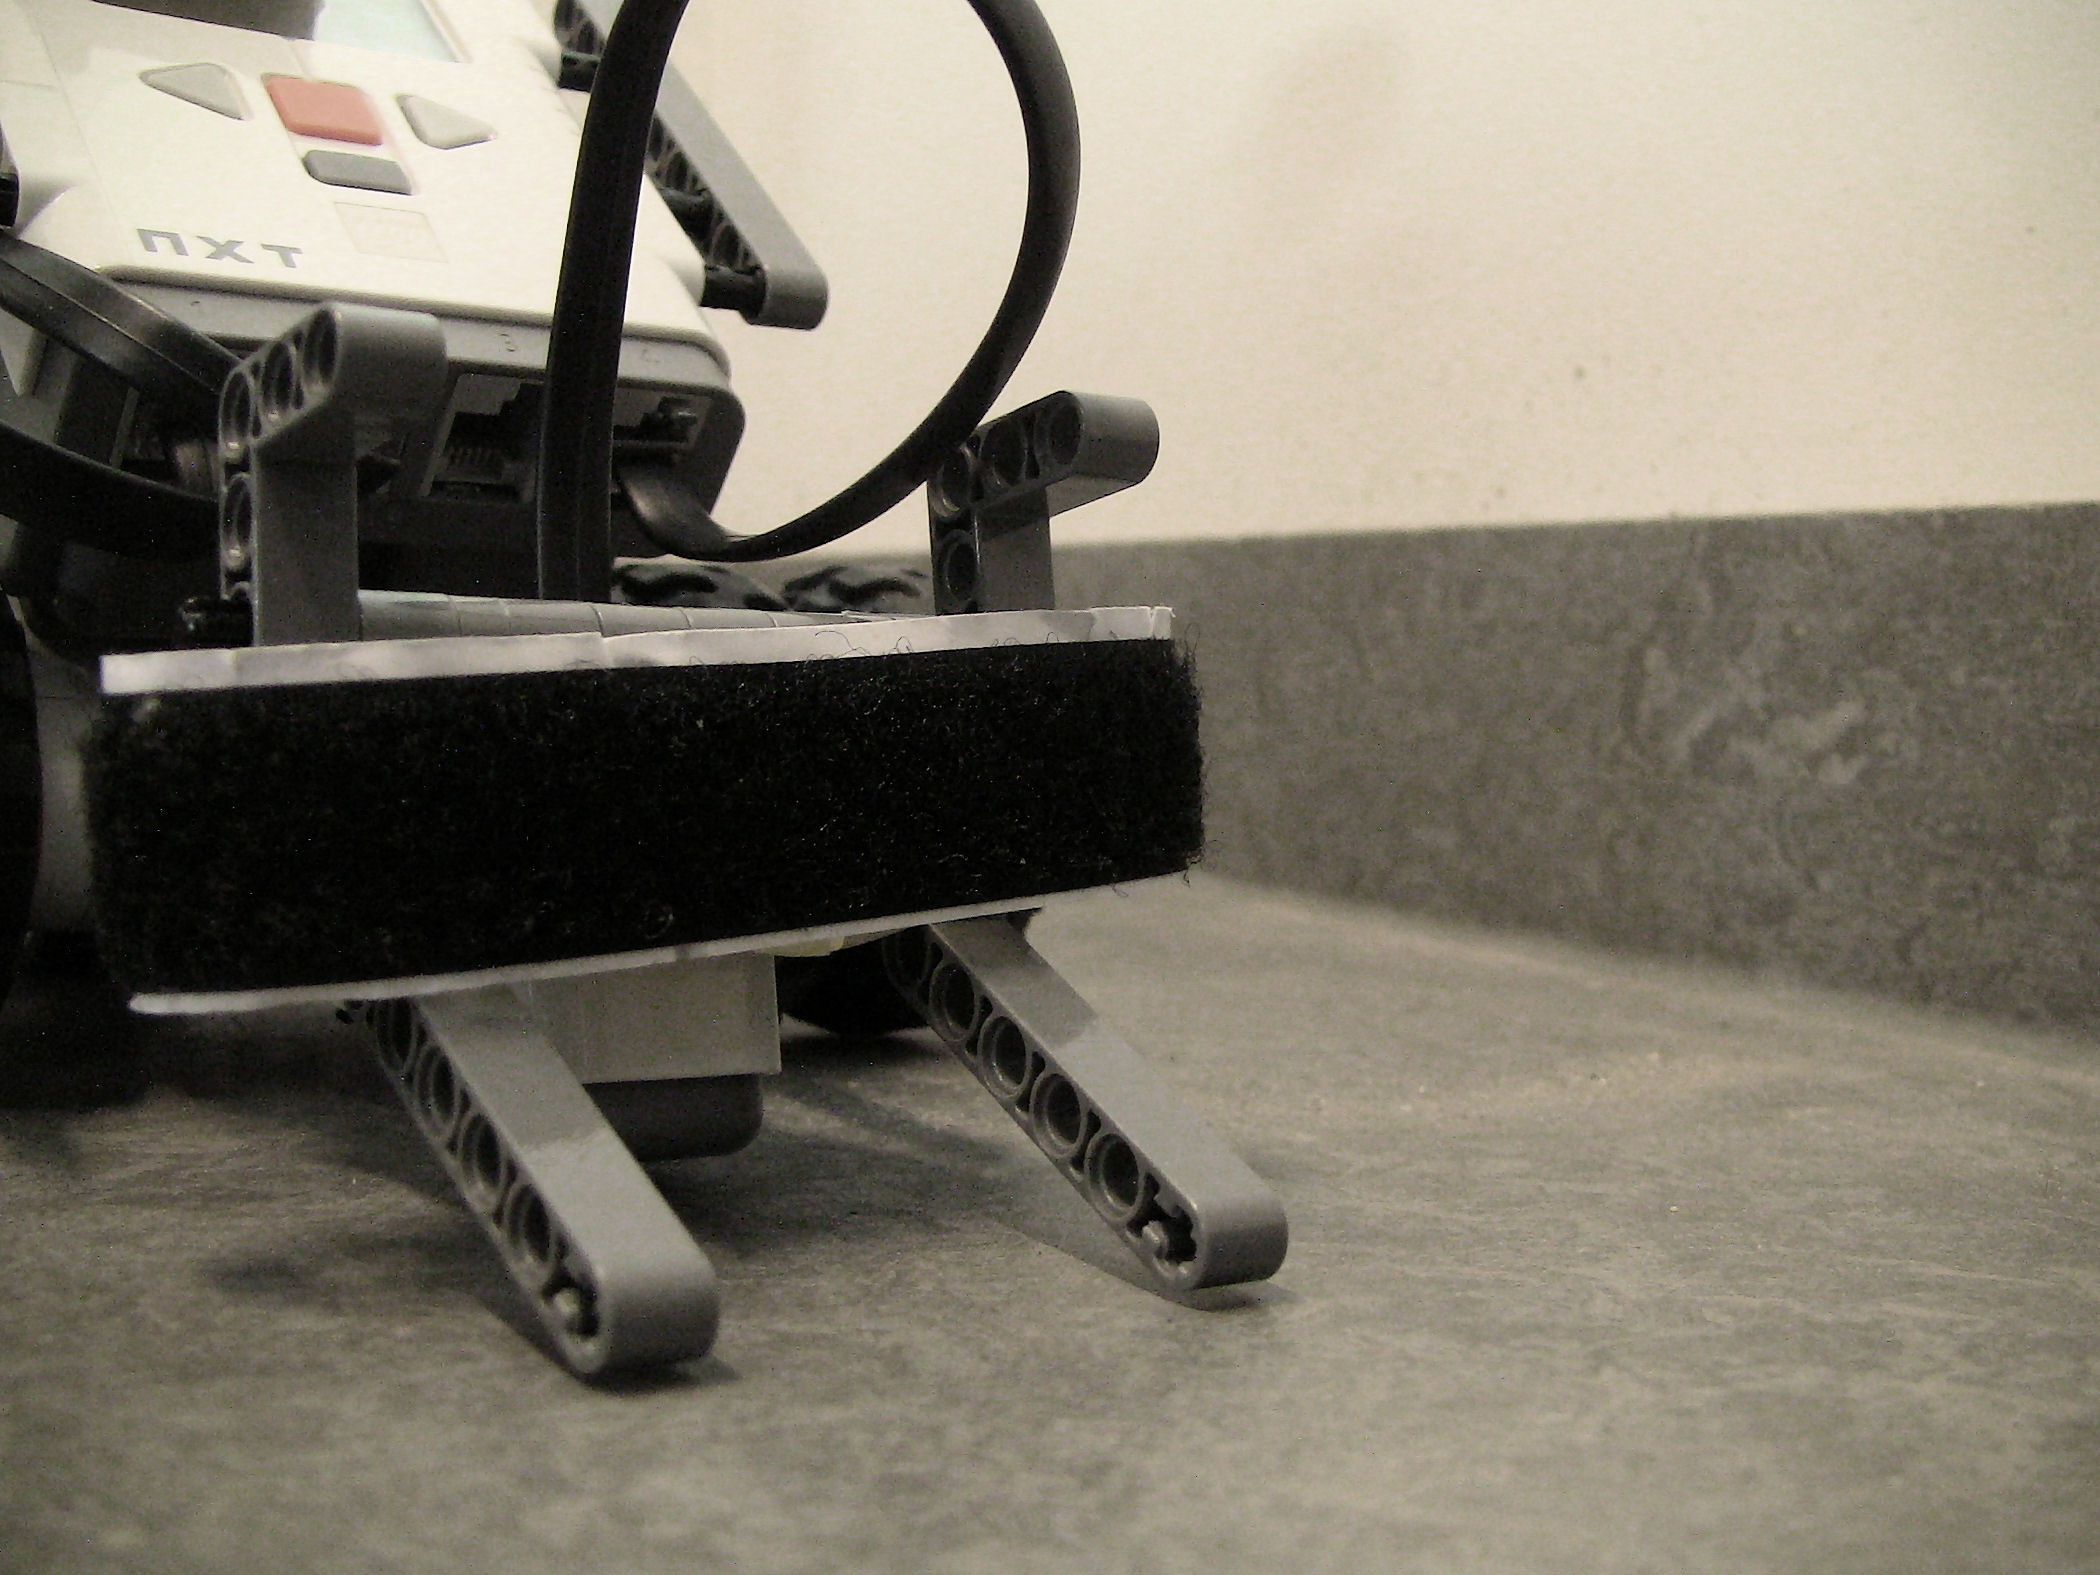
\includegraphics[width=\textwidth]{robotSchep}
		\caption{schep}
	\end{subfigure}%
	\begin{subfigure}[h]{0.33\textwidth}
		\centering
		\includegraphics[width=\textwidth]{robotWielen}
		\caption{wielen}
	\end{subfigure}%
	\begin{subfigure}[h]{0.33\textwidth}
		\centering
		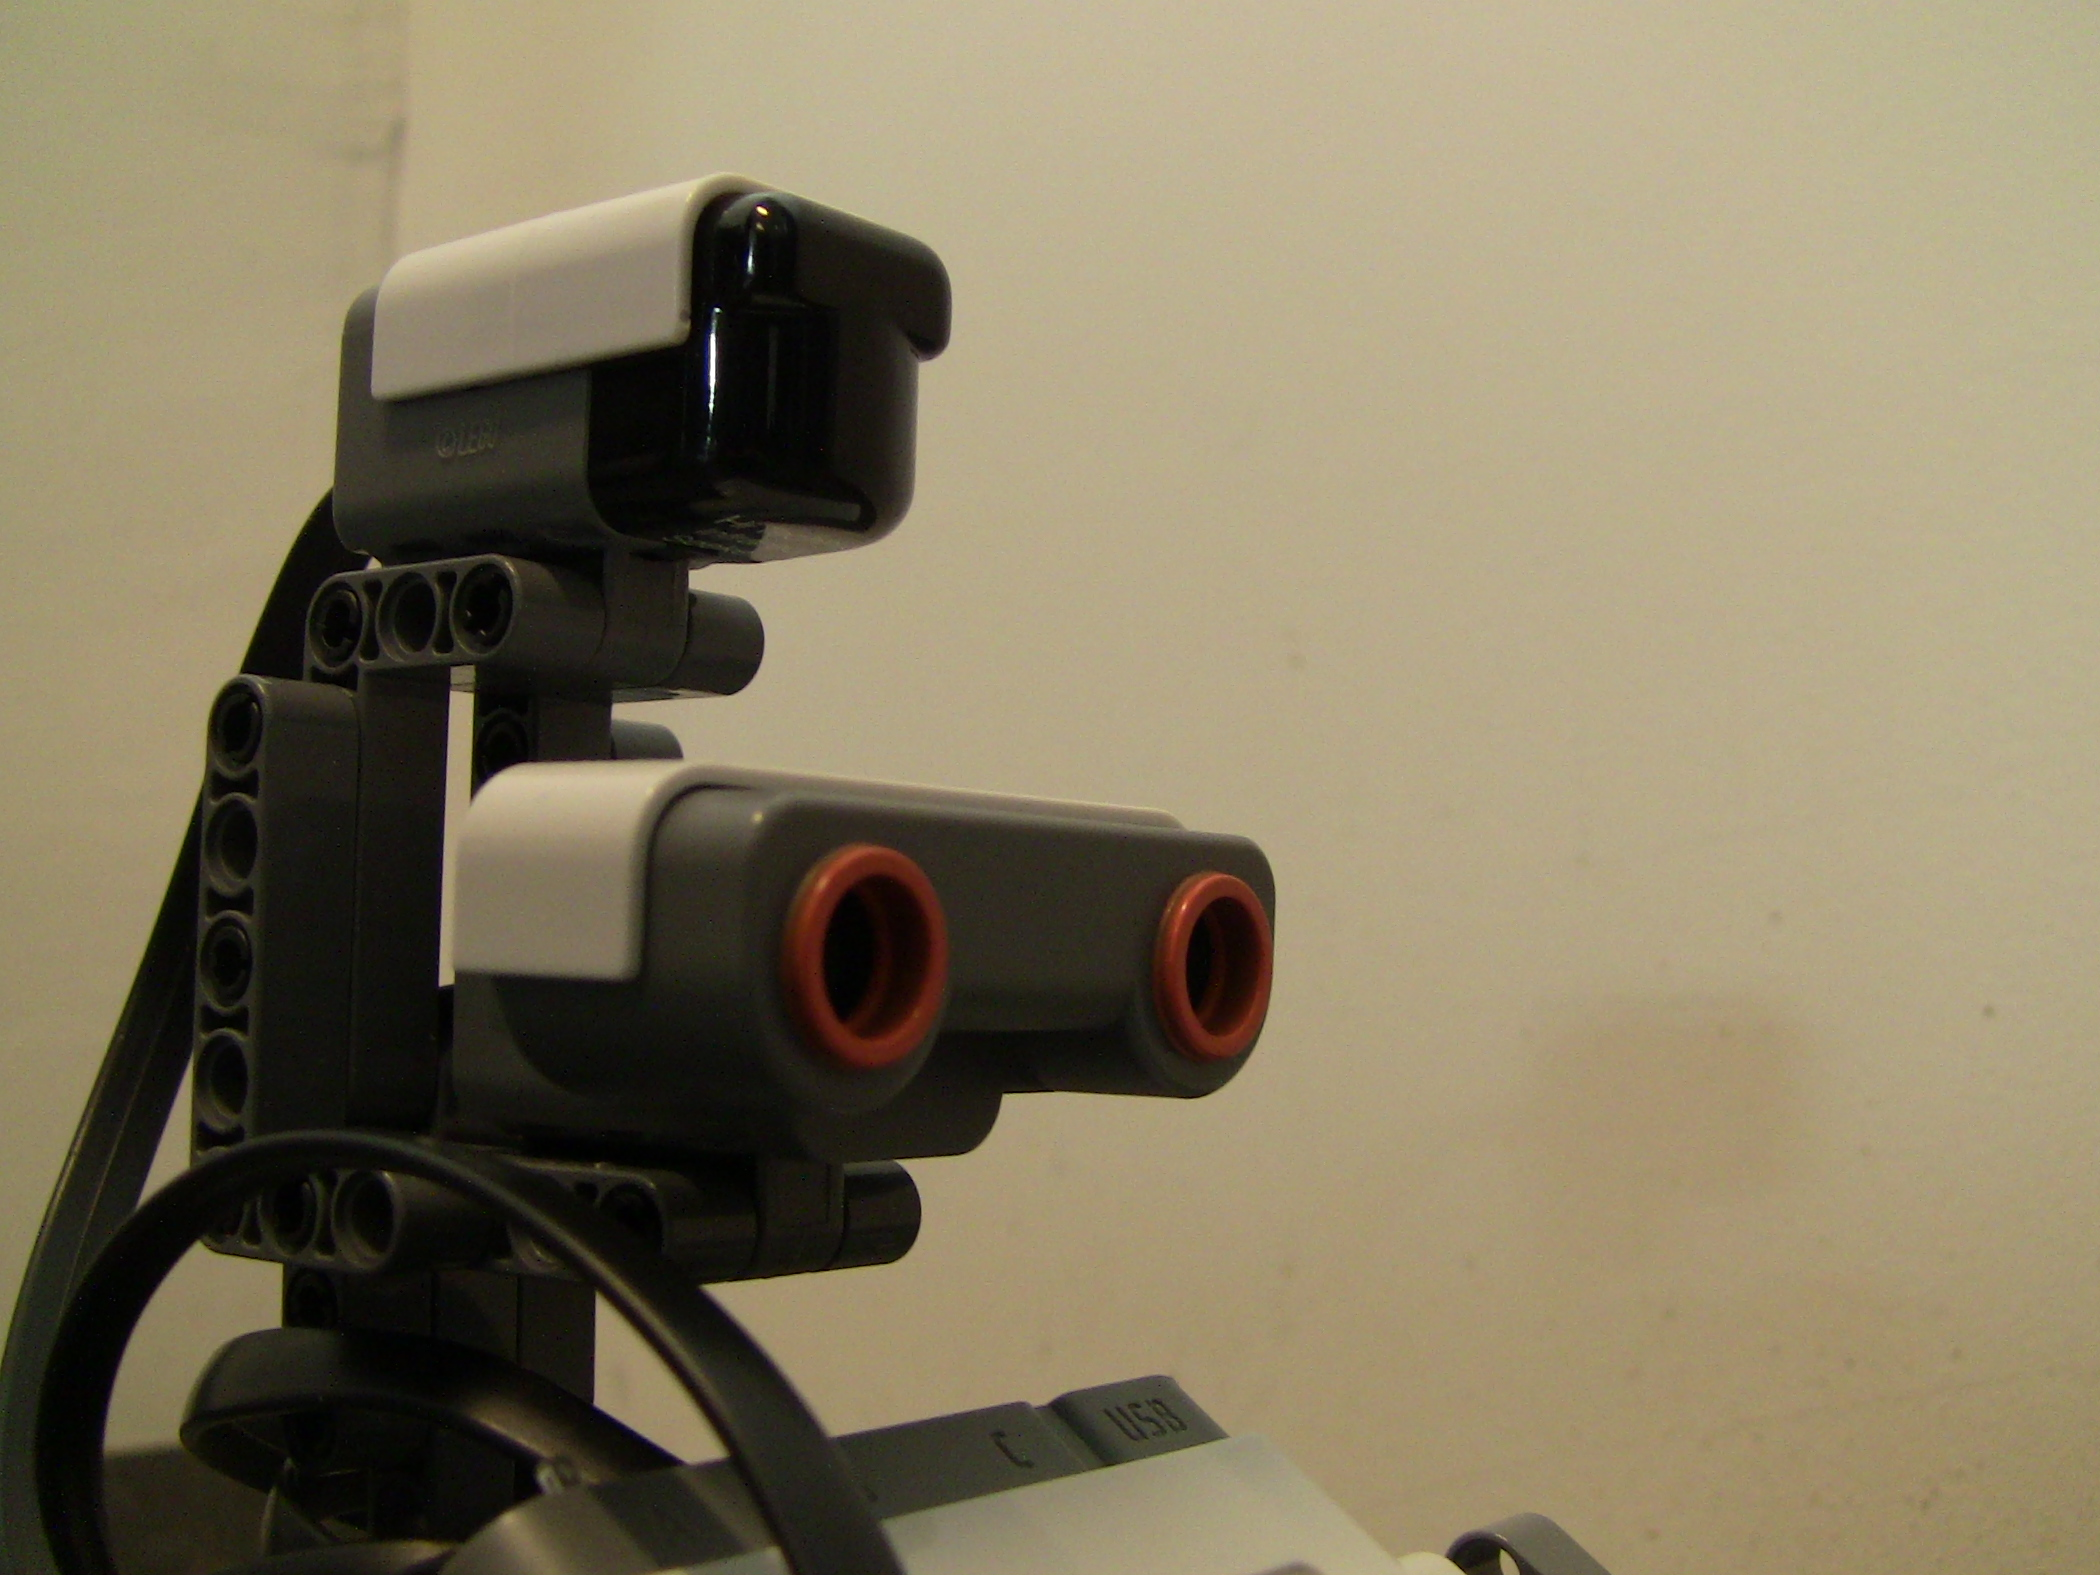
\includegraphics[width=\textwidth]{robotSensoren}
		\caption{infrarood- en ultrasone sensor}
	\end{subfigure}
\caption{Details van de robot.}
\label{fig:robotDetail}
\end{figure}


% == ALGORITMES == %
\section{Algoritmes}
Voor volgende algoritmes wordt verwezen naar het verslag van het eerste semester. Deze algoritmes worden dit semester zonder aanpassingen opnieuw gebruikt:
\begin{itemize}
	\item Rechtzetten op een witte lijn
	\item Centreren aan de hand van twee muren
	\item Lezen van een barcode
	\item Vinden van het kortste pad
\end{itemize}

% == zoeken van het voorwerp == %
\subsection{Zoeken van het voorwerp} %
\label{ssec:algoZoek}
Om het voorwerp te vinden moet de robot aanvankelijk het doolhof verkennen. De robot gebruikt hiervoor een implementatie van \textit{A*}. In de loop van het eerste semester werd dit algoritme geoptimaliseerd voor deze specifieke toepassing. Deze optimalisaties zijn ook dit semester van toepassing. \\
%TODO deze optimalisaties hierin zetten\\

\begin{description}
\item[A] basisalgoritme zonder optimalisatie: draai bij elke tegel vier keer (eindig in startori\"entatie) en neem de laatste tile in de queue als volgende tile.
\item[B] neem steeds de buur die met het minst aantal rotaties bereikt kan worden als volgende tile.
\item[C] draai bij elke tegel slechts drie keer (eindig niet meer in startori"entatie).
\item[D] muren die vanuit een naburige tile reeds gedetecteerd werden, worden niet nog eens nagekeken.
\item[E] tiles waarvan de vier zijden al gekend zijn en waaraan drie muren grenzen, worden niet meer bezocht (`dead-ends' kunnen onmogelijk barcodes bevatten, dus dit is geen probleem)
\end{description}

DeadEnd prioriteit

Er wordt een extra queue bijgehouden die de vakjes waar de robot nog niet weet hoe heen te gaan
omdat daar het doolhof nog niet verkend is bijhoudt. Wanneer hier een vakje in zit dat een deadend
is en wanneer er voor dat vakje mogelijk een straight in de juiste orientatie kan liggen, krijgt dit
vakje prioriteit en gaat de robot zo snel mogelijk naar daar manoeuvreren. Dit gebeurt door naar het
vakje te gaan dat wel bereikbaar is en dat zo dicht mogelijk ligt bij de deadEnd (zo klein mogelijke
manhattan distance).

Testen...

Uit deze testen blijkt dat het algoritme vaker efficienter is zonder deze optimalisatie. Dit komt omdat
de robot veel omrijdt om het dichtsbijzijnde vakje te vinden en daardoor meermaals hetzelfde pad
op en afgaat (een duidelijk voorbeeld hiervan is doolhof2 : .... ). Bij het oorspronkelijke algoritme was
dit meermaals over dezelfde wegen rijden heel hard geminimaliseerd.

Uit deze resultaten hebben we besloten om de optimalisatie niet door te voeren maar het
oorspronkelijke algoritme te behouden.

%
%Eerst werd er geopteerd om een extra optimalisatie (F) geeft prioriteit aan het vinden van het voorwerp. Een voorwerp kan zich enkel bevinden op een `dead-end', voorafgegaan door een `straight' met een barcode. Deze barcode identificeert het voorwerp. Wanneer een mogelijke voorwerp-locatie gevonden wordt, wordt zo snel mogelijk nagegaan of het om het juiste voorwerp gaat. In sommige gevallen is het niet mogelijk rechtstreeks naar de locatie te gaan omdat het doolhof daar nog niet verkend is. In dat geval wordt verder verkend in de richting van de locatie. De `dead-end' zelf hoeft niet bezocht te worden wanneer uit de barcode blijkt dat het niet om het juiste voorwerp gaat, zodat optimalisatie E nog steeds geldt.\\

Nadat het voorwerp gevonden is, probeert de robot zijn teamgenoot te contacteren. Indien de teamgenoot zijn voorwerp nog niet heeft of wanneer de mappen van beide robots nog niet combineerbaar zijn, gaat de robot verder met het verkennen van het doolhof. Hierbij wordt nog steeds prioriteit gegeven aan voorwerp-locaties. Deze bevatten immers unieke barcodes die het later gemakkelijker maken de mappen te combineren.

Als alternatief kan de robot zich naar het voorwerp van de teamgenoot begeven om daar op hem te wachten (niet te dichtbij om niet in de weg te staan). Deze extra optie wordt voorlopig nog niet ge\"implementeerd omdat nog niet duidelijk is in welke gevallen de strategie het best werkt.


\subsection{Weg vinden naar andere robot}
Hierbij dachten we aan het kortste-pad-algoritme. Dit zal wel nog aangepast moeten worden aan zowel draaien als vooruit rijden (draaien was nog niet in rekening gebracht).\\ Er moet ook nog rekening gehouden worden als de andere robot zou wegrijden. De robot mag hierdoor niet in een loop terechtkomen. Er zou moeten gecommuniceerd worden wie naar wie toerijdt, of dat er naar een gezamenlijke tegel moet gereden worden. \\
Als de andere robot zou wegrijden zou er een afstand kunnen bijgehouden worden die dan opnieuw berekent wordt als de afstand niet kleiner wordt.

% == SOFTWARE == %
\section{Software}
\label{secc:softw}

Bij het aanvatten van het tweede semester bleek dat de code van het project niet goed gestructureerd was. Het project is daarom grondig hervormd, opgekuist en ontward. Hier is veel tijd naar gegaan, maar we geloven dat het een nuttige investering is.\\

De software bestaat uit twee delen: een project dat op de NXT van de robot loopt en een project dat op de computer loopt (sectie \ref{ssec:Sdesign}). Alles wordt aangestuurd via de \textit{Graphical User Interface (GUI)} (sectie \ref{ssec:GUI}). Deze laat toe de robot te besturen en de reacties van de robot weer te geven. Robots kunnen met elkaar communiceren via RabbitMQ (sectie \ref{ssec:RabbMQ}). Via de GUI kunnen ook virtuele robots aangestuurd worden: de simulators (sectie \ref{ssec:Sim}).\\

Voor volgende secties wordt verwezen naar het verslag van het eerste semester. Deze implementaties en ontwerpen werden zonder aanpassingen opnieuw gebruikt:

\begin{itemize}
\item Commando's doorgeven
\item Bluetooth
\item Robot
\item Mappen van een doolhof
\end{itemize}

% -- Ontwerp -- %
\subsection{Ontwerp van het computerproject}
\label{ssec:Sdesign}
Een overzicht van het ontwerp wordt weergegeven in de klassendiagramma van figuur \ref{fig:klasDia}.\\

% figuren klassendiagramma
\begin{landscape}
\begin{figure}
\centering
	\begin{subfigure}{0.60\textwidth}
	\centering
		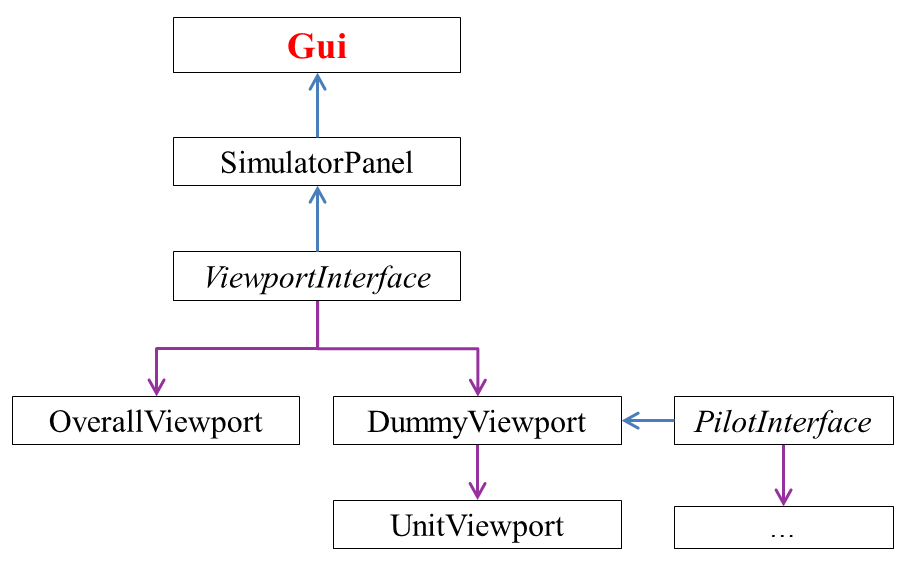
\includegraphics[width=\textwidth]{KlasGUI}
		\caption{GUI, SimulatorPanel en Viewports}
	\end{subfigure}%
	\begin{subfigure}{0.5\textwidth}
		\centering
		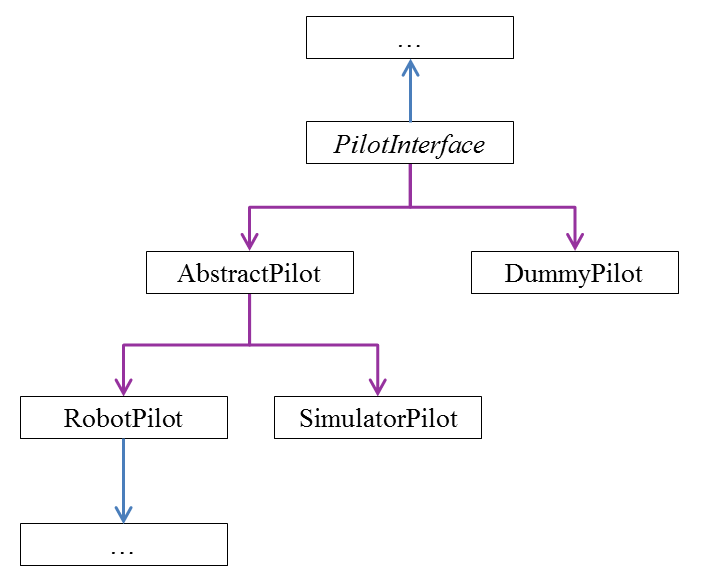
\includegraphics[width=\textwidth]{KlasPilot}
	\caption{Pilots}
\end{subfigure}%
\begin{subfigure}{0.45\textwidth}
		\centering
		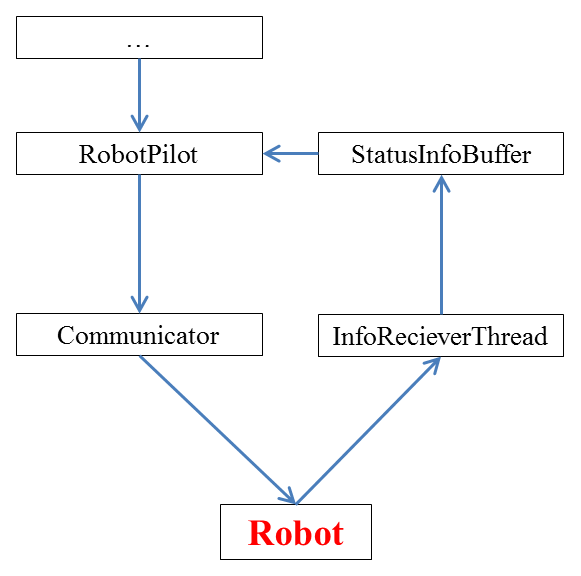
\includegraphics[width=\textwidth]{KlasRobot}
	\caption{Robot}
\end{subfigure}
\caption[Klassendiagramma]{Klassendiagramma (paarse pijlen wijzen op overerving of implementatie, blauwe op een informatiestroom)}
\label{fig:klasDia}
\end{figure}
\end{landscape}

De Main-methode bevindt zich in de GUI-klasse. Deze maakt een \textit{SimulatorPanel}-object aan. Dit is een overkoepelend panel waarin meerdere \textit{Viewports} zitten. Een \textit{OverallViewport} geeft het volledige doolhof en alle robots erin weer. Dit kan uiteraard enkel wanneer een gekend virtueel doolhof gebruikt wordt en wanneer van alle robots genoeg informatie beschikbaar is. Een \textit{UnitViewport} geeft de wereld van \'e\'en robot (eventueel gesimuleerd) weer: de sensorwaarden en de muren die hij reeds ontdekt heeft. Een wereld waarvan niets geweten is, kan niet worden weergegeven. Dit is het geval voor robots van andere teams: zij worden niet weergegeven in de GUI, met uitzondering van de teamgenoot. Deze laatste stuurt wel zijn map door, maar niet zijn sensorwaarden en wordt gerepresenteerd door een \textit{DummyViewPort}. Het aantal \textit{Viewports} hangt af van het aantal gekende werelden. Deze verdeling wordt weergegeven in tabel \ref{tab:aantViewPorts}.\\

% tabel #viewports
\begin{table}
\begin{center}
    \begin{tabular}{ c | c | c || c | c | c }
    wij & wij & anderen & aantal & aantal & aantal\\
    fysiek & gesimuleerd & fysiek/gesimuleerd & OveralViewports & UnitViewports & DummyViewports\\ \hline \hline
    1 & 3 & 0 & 1 & 4 & 0\\
    0 & 4 & 0 & 1 & 4 & 0\\
    1 & 0 & 3 & 0 & 1 & 1\\
    0 & 1 & 3 & 0 & 1 & 1\\
    \end{tabular}
    \caption{Overzicht van het aantal en de soort \textit{Viewports}}
    \label{tab:aantViewPorts}
\end{center}
\end{table}

Een \textit{DummyViewport} zal aanvankelijk niet worden weergeven. Wie de teamgenoot van de robot is, wordt immers pas bekend wanneer beide leden van het team hun voorwerp gevonden hebben. Op dat moment zal het \textit{DummyViewport} verschijnen.\\

Elke \textit{Viewport} krijgt een eigen \textit{Pilot} toegewezen (behalve \textit{OverallViewport}, die krijgt er meerdere). Er zijn verschillende soorten \textit{Pilots} die elk een implementatie van \textit{PilotInterface} zijn. De keuze van \textit{Pilot} hangt af van het type robot. Een robot waarvan de wereld niet kan worden voorgesteld, krijgt geen \textit{Pilot}. Een teamgenoot (die we niet zelf simuleren) heeft een \textit{DummyPilot}. Deze bevat enkel `getters', want deze robot kan niet worden aangestuurd. Een robot die gesimuleerd wordt, heeft een \textit{SimulatorPilot}. Deze berekent zelf zijn sensorwaarden op basis van een virtuele doolhof. Een fysieke robot krijgt een \textit{RobotPilot} die via de \textit{Communicator} in verbinding staat met de fysieke robot. De \textit{RobotPilot} krijgt zijn sensorwaarden terug van de robot via de \textit{InfoReceiverThread} en de \textit{StatusInfoBuffer}. Deze \textit{Pilots} zijn de `hersenen' van deze robots/simulators. De \textit{Viewports} geven enkel weer wat de robots uitvoeren, zij berekenen en beslissen niets.

% -- GUI -- %
\subsection{Grafische User Interface}
\label{ssec:GUI}

% figuur GUI
\begin{figure}[h]
\centering
	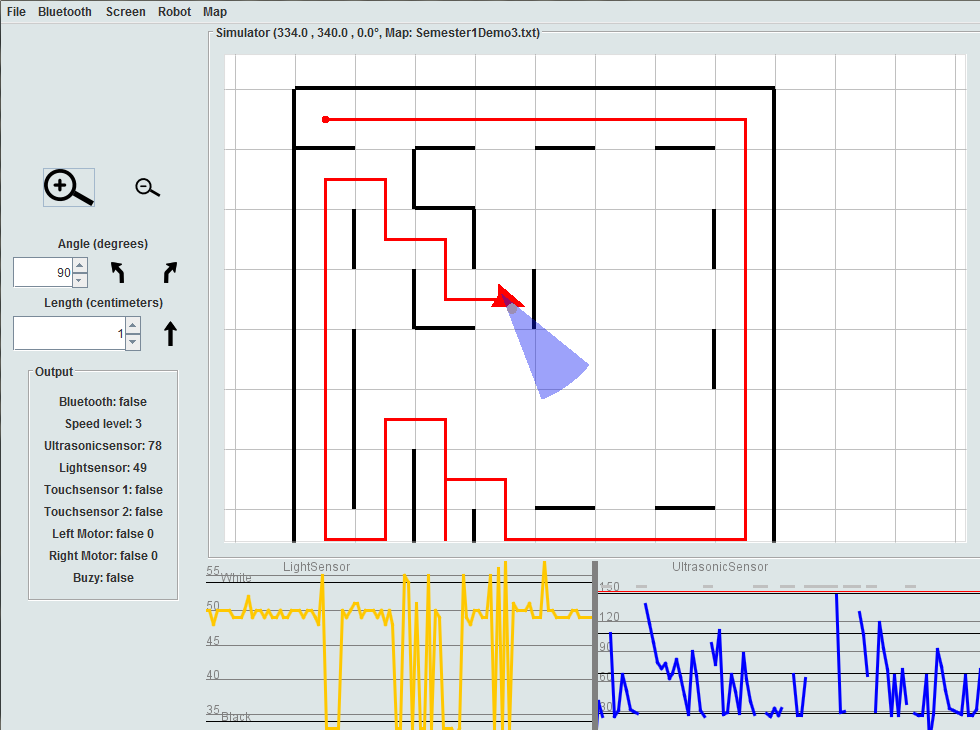
\includegraphics[width=0.8\textwidth]{GUI}
\caption{de Graphical User Interface}
\label{fig:GUI}
\end{figure}

De nieuwe GUI is nog niet volledig klaar. Een figuur van de GUI zoals deze er in het eerste semester uit zag, wordt weergegeven in figuur \ref{fig:GUI}.\\

De GUI zal er wat anders uitzien dan vorig semester. Het moet nu immers mogelijk zijn de wereld van meerdere robots tegelijk weer te geven. Deze werelden verschillen van elkaar: zeker in het begin verkennen de verschillende robots een ander deel van het doolhof. Omdat zowel beginpositie als -ori\"entatie niet gekend zijn, is het niet mogelijk al deze werelden in \'e\'en paneel weer te geven. Het \textit{SimulatorPanel} wordt opgedeeld in verschillende \textit{Viewports}. Zoals uitgelegd in sectie \ref{ssec:Sdesign} hangt het aantal \textit{Viewports} af van de situatie.\\

Wanneer de robot een pad aflegt, tekent de \textit{UnitViewport} dit in het tekenpaneel als een rode lijn (herschaald: \'e\'en cm = \'e\'en pixel). De lijnen worden als lijnen opgeslagen in de \textit{UnitViewport}. Wanneer de robot een rechte weg aflegt, wordt het eindpunt van de gedefinieerde lijn steeds verlegd. Dit zorgt ervoor dat de weg die de robot aflegt continu bijgewerkt wordt. De huidige positie en de huidige ori\"entatie van de robot worden weergegeven door een driehoek die draait met de ori\"entatie. Het bereik van de ultrasone sensor wordt grafisch weergegeven met een blauwe boog. De lichtsensor wordt voorgesteld als een bol die van kleur verandert wanneer de ondergrond wijzigt. 
Een \textit{DummyViewport} geeft geen pad of sensorwaarden weer, enkel een map. De map-in-opbouw wordt weergegeven op basis van de map die de \textit{Pilot} opstelt.\\

Al deze \textit{Viewports} nemen plaats in, waardoor andere functionaliteiten van de GUI naar de achtergrond moeten verdwijnen. De sensorgrafieken, bijvoorbeeld, zullen nog beschikbaar zijn, maar worden enkel zichtbaar wanneer deze via een menu expliciet geopend worden. Zo kunnen ze nog steeds gebruikt worden voor testen.



% -- RabbitMQ -- %
\subsection{RabbitMQ}
\label{ssec:RabbMQ}
De implementatie van RabbitMQ  is sterk gebaseerd op de demo die op Toledo werd geplaatst.\\

Elke \textit{AbstractPilot} moet kunnen interageren met een RabbitMQ-kanaal. De klasse \textit{MessageCenter} zorgt voor een RabbitMQ-interface die de pilots kunnen gebruiken. Het object verbindt met een server bij initialisatie. Enkele algemene parameters worden meegegeven: gebruikersnaam, wachtwoord en poort. De belangrijkste methodes in de klasse zijn \textit{sendMessage()} en \textit{subscribeTo()} die respectievelijk het schrijven naar en monitoren van, specifieke `exchanges' en `queues' toelaten. De methodes aanroepen heeft volgend effect:

\begin{description}
\item[subscribeTo(String monitorKey):] Een object van de klasse \textit{SubscribeMonitor} wordt aangemaakt. Deze \textit{SubscribeMonitor} luistert naar alle berichten op het kanaal van het \textit{MessageCenter} die met de gegeven string beginnen (de `Monitor Key'). Vervolgens stuurt het \textit{MessageCenter} al deze informatie naar de \textit{AbstractPilot} die de monitoring-aanvraag deed. Deze Pilot ontvangt vanaf dan alle berichten met het onderwerp waarvoor hij een aanvraag deed, maar van berichten met een ander onderwerp krijgt hij geen melding.
\item[sendMessage(String exchange, String routingKey, String message):] Het gegeven bericht wordt naar de gespecifi\"eerde `exchange' gestuurd. Deze plaatst het bericht in alle `queues' die het onderwerp (gespecifi\"eerd door de routingKey) volgen. Op deze manier krijgen alle \textit{Pilots} die aanvraag deden voor het onderwerp, melding van het bericht.
\end{description}

% De scheidsrechterscommissie ontwikkelde ‘Het Team Treasure Trek Protocol’ ofwel HTTTP. Het protocol voorziet in een breed scala van methodes: het starten, stoppen en pauzeren van een Game, het toewijzen van objecten, het melden van een locatie-wijziging, … Ook voorzag de commissie een implementatie. Daarin zit een Client-klasse die onder andere voorgenoemde methoden aanbiedt en die het gebruik van RabbitMQ bijna volledig abstraheert. 
%
%Elk team maakt zelf een implementatie van de bijgevoegde Handler-interface. Zo’n Handler zorgt ervoor dat de info die op de RabbitMQ-kanalen binnenkomt juist gebruikt wordt. In dit project bestaan er meerdere implementaties van die Handlers. Elk soort Pilot gaat immers anders met die info om. De Robot- en SimulatorPilots die instaan voor het besturen van Robots en Simulatoren gebruiken bijvoorbeeld de informatie voor het starten van een game, terwijl DummyHandlers informatie voeren aan de DummyPilots die andere Robots modeleren. Van daaruit is het dan makkelijker om aan mapmerging etc. te doen. Een overzicht van de voorziene architectuur zie je in figuur TODO
%
%Bij het aanmaken van een Pilot wordt er een MQCenter aangemaakt met bijhorende Handler. Dit MQCenter abstraheert verder de - reusachtige - Client-klasse en zorgt ervoor dat een AbstractPilot makkelijk htttp-ondersteuning krijgt.

% -- Simulator -- %
\subsection{Simulator}
\label{ssec:Sim}
De \textit{Simulator} bootst de werking van de robot virtueel na. Hij kan dezelfde commando's uitvoeren als de werkelijke robot en simuleert de sensorwaarden die een echte robot zou genereren wanneer deze zich in een soortgelijke situatie bevindt.\\

De \textit{SimulatorPilot} bepaalt de positie van de `robot' ten opzichte van het virtuele doolhof: hoe ver van de muur en op welke ondergrond. De klasse \textit{SimulationSensorData} houdt sensorwaarden bij van tests op de echte robot in verschillende situaties. De \textit{SimulatorPilot} haalt hier zijn referenties uit en probeert op basis van de meetwaarden een realistische sensorwaarde te genereren. De sensorwaarden worden niet nauwkeurig gegenereerd: er wordt ruis toegevoegd. De echte robot geeft immers ook geen exacte waarden.\\

De \textit{AbstractPilot} bepaalt hoe de gesimuleerde robot moet reageren in de gegeven situatie. De klasse bevat methodes als \textit{travel()} en \textit{rotate()}. Ook bouwt de \textit{AbstractPilot} een map op terwijl de robot zich voortbeweegt door het doolhof. De \textit{AbstractPilot} kan zowel de echte robot als een gesimuleerde robot aansturen. De \textit{AbstractPilots} zijn de hersenen van de robots.


% == BESLUIT == %
\section{Besluit}
De bouw van de robot wordt uitgebreid met een infraroodsensor bovenaan en een schep vooraan. De schep laat toe een voorwerp op te rapen. Op de schep is klittenband aangebracht zodat het voorwerp stevig vastzit. De lichtsensor heeft een scharnier gekregen. Zo zit de lichtsensor niet in de weg wanneer de robot over een wip rijdt. \\

De GUI ziet er anders uit dan vorig semester. Zo kunnen nu ook de tegenstanders en de teamgenoot gesimuleerd worden. Al deze robots (al dan niet gesimuleerd) hebben een eigen idee van de wereld. Deze verschillende werelden worden weergegeven via \textit{Viewports}.\\

Verder werd de communicatie ge\"implementeerd zodat de robot een bericht kan sturen wanneer hij zijn voorwerp vindt. 
De robot communiceert met andere robots via RabbitMQ. Zo kan de robot afspraken maken met anderen en kan hij te weten komen wie zijn teamgenoot is.
 


\newpage
\makeappendix

%% == DEMO 1 == %
\section{Demo 1} % 3
\label{Asec:demo1}
De robot wordt voor de eerste demo voorzien van een schep die bestaat uit een halve wc-rol. De infraroodsensor is ge\"installeerd, maar wordt nog niet gebruikt. Wanneer de robot zijn voorwerp vindt, stuurt hij een bericht via RabbitMQ. De GUI is opgesplitst in verschillende \textit{Viewports} die elks \'e\'en of meerdere \textit{Pilots} weergeeft.

% == resulaten == %
\subsection{Resultaten} % 3 ?
\label{Assec:result1}
Het algoritme waarmee de robot zijn voorwerp opraapte, maakte gebruik van de travel() methode. De \textit{ExploreMaze}-thread wist echter niet dat de robot van plek was verandert. In de waan dat de robot op een andere plek stond dan in werkelijkheid, gaf de thread verkeerde instructies waardoor de robot tegen een muur reed. \\
Het schepsysteem van de robot functioneerde niet zo goed. Tijdens de demo faalde de robot toen hij het object moest oprapen. 

% == conclusies == %
\subsection{Conclusies} % 3 ?
\label{Assec:conc1}
Het bovengenoemd probleem is voor de volgende demo opgelost. Wanneer de \textit{ExploreMaze}-thread onderbroken wordt, zorgt de onderbrekende methode steeds dat de robot op dezelfde plek staat als waar de \textit{ExploreMaze}-thread denkt dat de robot staat.\\
Het opraapsysteem voor de robot is ook aangepast. De schep is weggehaald en er is een velcrostrip aangebracht. De robot is nog steeds in staat om het voorwerp met een liftsysteem op te heffen, zodat de robot vlot over de wip heen kan.


% == aanpassingen == %
\subsection{Oplijsting aanpassingen verslag} % 3 ?
\label{Assec:aanp1}
Volgende secties werden aangepast ten opzichte van de eerste demonstratie:

% overzicht aangepaste secties
\begin{itemize}
\item \textit{\ref{ssec:fysb} Fysieke bouw:} de schep vooraan werd aangepast.
\item \textit{\ref{ssec:algoZoek} Zoeken van het voorwerp:} testen van de prioriteit.
\item \textit{\ref{ssec:infra} Infraroodsensor:} Nieuw stuk over infraroodsensor werd toegevoegd, samen met de testen.
%\item \textit{calibratie infrarood}: nieuwe gegevens.
\end{itemize}

\newpage

%\begin{thebibliography}{9}
%
%\bibitem{TeamTreasure} 
%\textit{Team Treasure Trek}: Een onderdeel van Mario Party 4. \mbox{[www.nintendo-europe.com/]}
%
%\bibitem{RabbitMQ}
%\textit{RabbitMQ}: Een communicatiesysteem dat het Advanced Message Queing Protocol (AMQP) implementeert. Door een kanaal op te zetten met een RabbitMQ-server is het mogelijk een bericht te plaatsen dat anderen kunnen lezen. De server heeft enkele `exchanges' die de berichten verdelen over `queues'. Die `queues' worden aangemaakt door de `clients' en luisteren elk naar een bepaald onderwerp. De `exchange' pushed dus berichten met een bepaald onderwerp naar de juiste `queues'.
%\mbox{[http://en.wikipedia.org/wiki/RabbitMQ]}
%
%\bibitem{mindstorms}
%\textit{Lego Mindstorms}:  Een uitbreiding op de LEGO bouwstenen waarmee kleine, aanpasbare en programmeerbare robots gebouwd kunnen worden. Een centrale besturingsmodule (`the brick') kan geprogrammeerd worden met verschillende programmeertalen. In eerdere versies werd een RCX gebruikt voor de brick, nu wordt met NXT gewerkt. De brick kan enkele motoren aandrijven. Bovendien kunnen er verschillende sensoren, o.a. een ultrasone sensor en een lichtsensor, aangesloten worden.  \mbox{[www.lego.com]} \mbox{[http://en.wikipedia.org/wiki/Lego\textendash Mindstorms]}
%
%\bibitem{leJOS}
%\textit{leJOS}: Een kleine Java Virtuele Machine die toelaat de NXT-brick te programmeren. leJOS voorziet verschillende klassen die o.a. de motoren aansturen en een bluetoothverbinding opzetten.  \mbox{[http://lejos.sourceforge.net/]}
%
%
%
%\end{thebibliography}


\end{document}
